\chapter{Results}
\label{chap:results}

\section{Overview}
\label{sec:results-overview}


Revised Content with Chapter Structure
Chapter 4: Results and Evaluation

In this chapter, I present the evaluation results of both agent and tool routers. First, I'll outline the testing framework that provided a controlled environment for assessment. While the AI generated testing data may not perfectly mirror real world scenarios, it establishes a consistent baseline for performance measurement. I'll analyze the pass/fail/warn rates for both router types and discuss what these metrics reveal about their operational reliability.

Having implemented these routers as an OpenWebUI plugin, I'll share insights from the integration process. This section examines the technical challenges encountered, adaptation requirements, and overall implementation complexity. I'll provide a candid assessment of how smoothly the routers integrated into an existing ecosystem and what developers should anticipate when adopting similar solutions.

This section evaluates the routers' performance in production conditions using my self-hosted OpenWebUI instance. I'll compare the operational benefits against implementation costs to determine if routers deliver meaningful advantages in real-world applications. The analysis includes benchmarking against alternative NLI models to provide context for decision-making.

For fine-tuned models, I'll analyse performance metrics compared to their base versions. This includes examining accuracy improvements, response quality, and resource efficiency. I'll document challenges encountered during the fine-tuning process, solutions developed, and opportunities for future optimization.

The final section provides a comprehensive assessment of router technology as a productivity enhancement tool. I'll examine whether implementation efforts translate to meaningful improvements in operational efficiency. Additionally, I'll explore alternative architectural approaches beyond NLI that might deliver similar or superior benefits in certain contexts.


\subsection{Test Results}
\label{sec:results-overview}

Using the testing script from the previous chapter, For every test prompt from the synthetic data, the router will select a Agent and a Tool best suited to handle the prompt. The results are recorded as either a pass, fail, or warn. 

As shown in the plot below, The tool router performed significantly better than the agent router where out of 70 test prompts, the tool router had a pass rate of 45, 18 warns, and only 7 fails. The agent router, on the other hand, performed significantly worse with a pass rate of 28, 13 warns, and 29 fails. 

As illustrated in Figure \ref{fig:router-results},  with a total of 70 test prompts:
\begin{itemize}
    \item The tool router had a pass rate of 45, 18 warns, and only 7 fails.
    \item The agent router had a pass rate of 28, 13 warns, and 29 fails.
\end{itemize}

The results indicate that the tool router was more effective in selecting the appropriate tool for the given prompts, while the agent router struggled, Although this could be significantly improved if the description of the agents were tweaked to be more descriptive and specific to the task at hand. 

\begin{figure}[H]
    \centering
    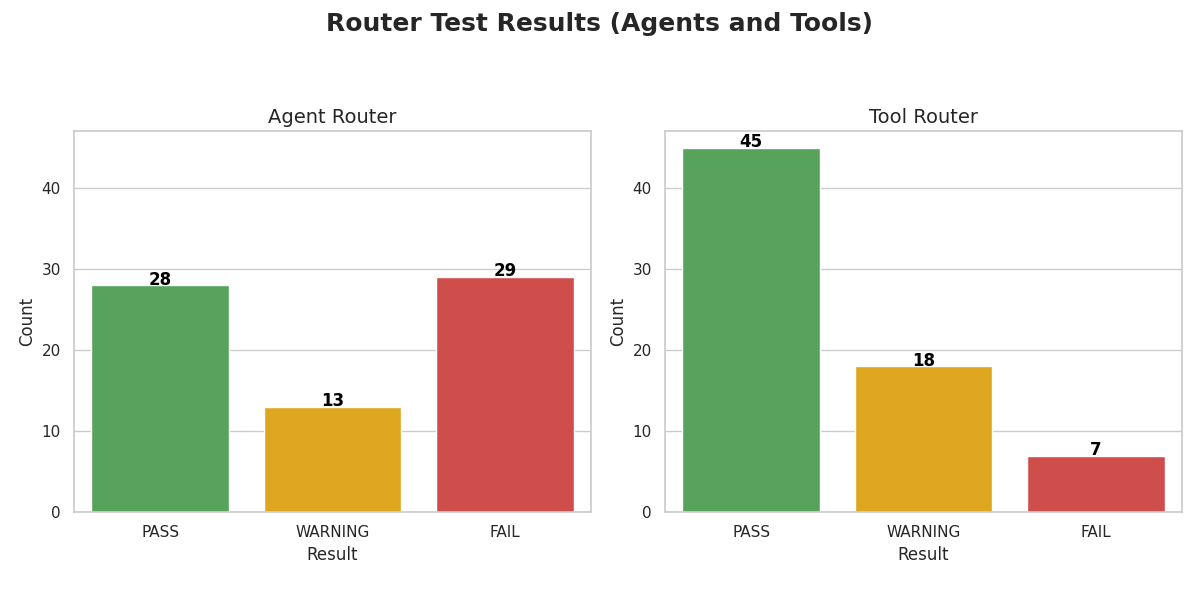
\includegraphics[width=0.8\textwidth]{figures/plots/router_test_summary.png}
    \caption{Router Performance Results}
    \label{fig:router-results}
\end{figure}



\begin{figure}[H]
    \centering
    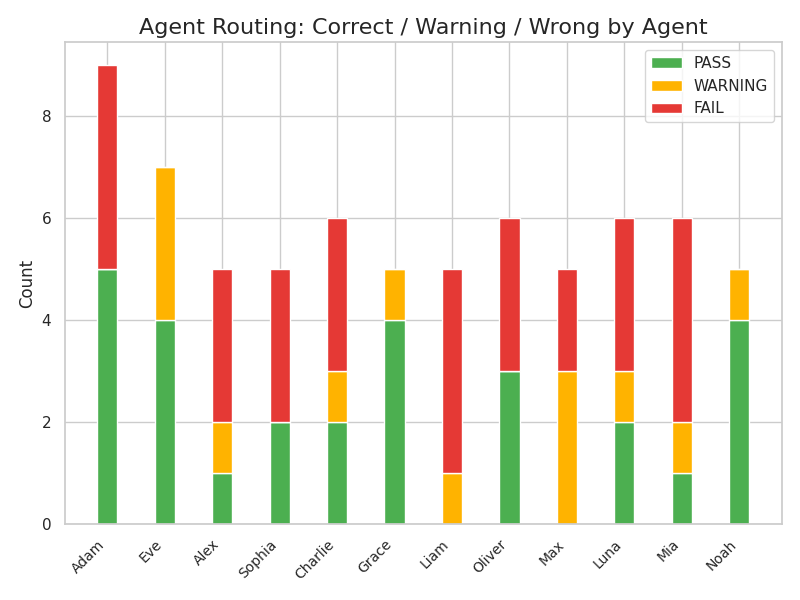
\includegraphics[width=0.8\textwidth]{figures/plots/agent_routing_per_agent.png}
    \caption{Agent Router Performance Results}
    \label{fig:agent-router-results}
\end{figure}

\begin{figure}[H]
    \centering
    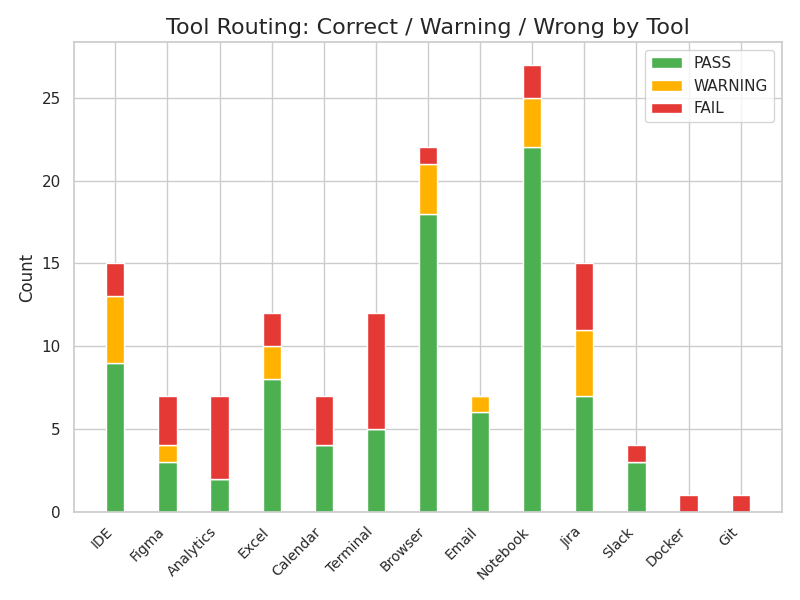
\includegraphics[width=0.8\textwidth]{figures/plots/tool_routing_per_tool.png}
    \caption{Tool Router Performance Results}
    \label{fig:tool-router-results}
\end{figure}

\begin{quote}
    \textbf{Scoring System:}
    \textit{
    \begin{itemize}
        \item Pass: The router selected the correct agent or tool for the task.
        \item Warn: The router selected an agent or tool that was not the best fit, but was within the top 3 candidates.
        \item Fail: The router selected an agent or tool that was not within the top 3 candidates.
    \end{itemize}
    }
\end{quote}

\subsection{Performance}
\label{sec:results-performance}

The pipeline functionality of this router seems to clasify the task almost instantly. This might be due to the fact that its using A GPU to run the NLI model. Besides the initialisation of the fist router, which took a few milliseconds, the router was able to classify the task in less than 0.1 seconds. This is significantly faster than if the router based its decision on the output of the LLM. Additionally, testing on CPU might be required to see if the performance is still acceptable.

\subsubsection{How to Improve the Router}
\label{sec:results-improve-router}

As shown in the results, the agent router performed significantly worse than the tool router. This could be improved by tweaking the descriptions of the agents to be more descriptive and specific to the task at hand. For example, instead of just saying "I am a translator", the agent could say "I am a translator who specializes in legal documents". This would help the router to better understand the capabilities of each agent and select the most appropriate one for the task. Additionally, the agent router could be improved by providing the output from the tool router as input to the agent router. This would allow the agent router to get contextual of the task at hand and select the most appropriate agent for the task.

Another way to improve the agent router is to use a fine-tuned model that is specifically designed for routing tasks. As mentioned in the previous chapter, fine-tuning \textit{can improve} the reliability of the model. This could be done by training the model on a dataset of routing tasks, where the model learns to select the most appropriate agent for each task. This would require a significant amount of data and computational resources, but it could lead to an improvement.

\section{Experience with Implementing Routers into OpenWebUI}
\label{sec:results-implementation}
As mentioned in the development chapter, although the documentation for OpenWebUI was quite sparse, I was able to implement all three routers into the OpenWebUI framework. The implementation process was relatively straightforward, as the framework provided a clear structure for adding new components. However, I did encounter some challenges along the way. The most significant challenge was that I could not find a way of getting a list of all available agents even though the framework provided a way to get a list of all available tools. This meant that I had to hardcode the list of agents into the router, which made it less flexible and more difficult to maintain. 

making the router llm library a simple python package that can be installed via pip made the implementation process much easier. This allowed me to easily import the router library into the OpenWebUI framework and use it without having to worry about dependencies or compatibility issues.

\subsection{Developer Experience}
\label{sec:results-developer-experience}
The implementation of the routers into OpenWebUI was a relatively smooth process, thanks to OpenWebUI's function feature that lets you modify the chat object before and after inference. In terms of developer experience, making the \texttt{router\_llm} library a simple Python package greatly helped with the implementation process, as mentioned previously. Additionally, the library was designed to simply initialise the router and pass the user input to it, making it trivial to implement for any other UI applications that allow for customisation of the chat object.


\subsection{User Experience}
\label{sec:results-user-experience}

The user experience of the routers was generally positive. Although inicially, the route was horibly slow, after some optimisations, such as using multi-threading and adding batching, the routers were able to process requests much faster.

The user interface of OpenWebUI was also well-designed, making it easy for users to interact with the routers for example, the tool router will show a spinner while looking for a tool and update the UI with the selected tool with a probability score. This made it easy for users to understand what was happening behind the scenes and how the routers were making their decisions.

\subsection{Production Viability Assessment}
\label{sec:results-production-viability}

Since I found the implementation of the routers into OpenWebUI to be relatively straightforward, I believe that the routers are at least beta ready. However, there are still some areas that need to be improved before they can be considered for production use. For example, a Fine tuning model for both the agent and tool routers would greatly improve the performance of the routers. Additionally, the routers need to be tested in a production environment to ensure that they can handle the load and scale as needed since the current implementation was only tested on a single machine.

\section{Fine-tuning Outcomes and Improvements}
\label{sec:results-fine-tuning}

Although I did try to fine-tune the models, I was not able to get the results I was hoping for. The main issue was that the models were not able to learn from the data I provided. This could be due to a number of factors, such as quality of the data, the size of the dataset, or the complexity of the task. I believe that with more time and resources, I could have achieved better results. Additionally, I did not have access to compute resources that would allow me to train the models for a longer period of time. However, I was able to learn a lot from the process and I believe that fine-tuning is a valuable tool for improving the performance of models. I have provided the models In the github repository along with the jupyter notebooks used to train them. I believe that with more time and a better selection of data, It could be possible to achieve better results.

\subsection{Fine-tuning Results}
\label{sec:results-fine-tuning-results}


As seen in the outputs of the jupyter notebooks, although showing a low training loss, the models were not able to learn from the data I provided. In the future, I would recommend using a larger dataset with more diverse examples to help the models learn better. Although the fine-tuning process was not successful, trying to fine-tune the models was a valuable learning experience.


\subsection{Overall Effectiveness}
\label{sec:results-effectiveness}

Although the routers were able to classify the tasks It did struggle with some prompts. The main issue was when the prompt was too vague or required additional context. As stated in the previous chapter, this could be improved by imporving the descriptions of the agents and tools. Or further changing the way the router are called for instance, providing the output of the tool router as input to the agent router. To further improve the performance of the routers, I would recommend fine-tuning the models with a larger dataset that is more representative of the tasks that the routers will be used for would also help improve the performance of the routers.



